\chapter{HASIL DAN PEMBAHASAN}

\section{Hasil Rancangan Sistem Identifikasi Kendaraan Pada Pemarkiran Dengan Pengenalan Citra Dan Pembacaan RFID}

\subsection{Hasil Perancangan Perangkat Keras}

\subsection{Raspberry Pi dan RFID MFRC522}
\begin{figure} [H]
    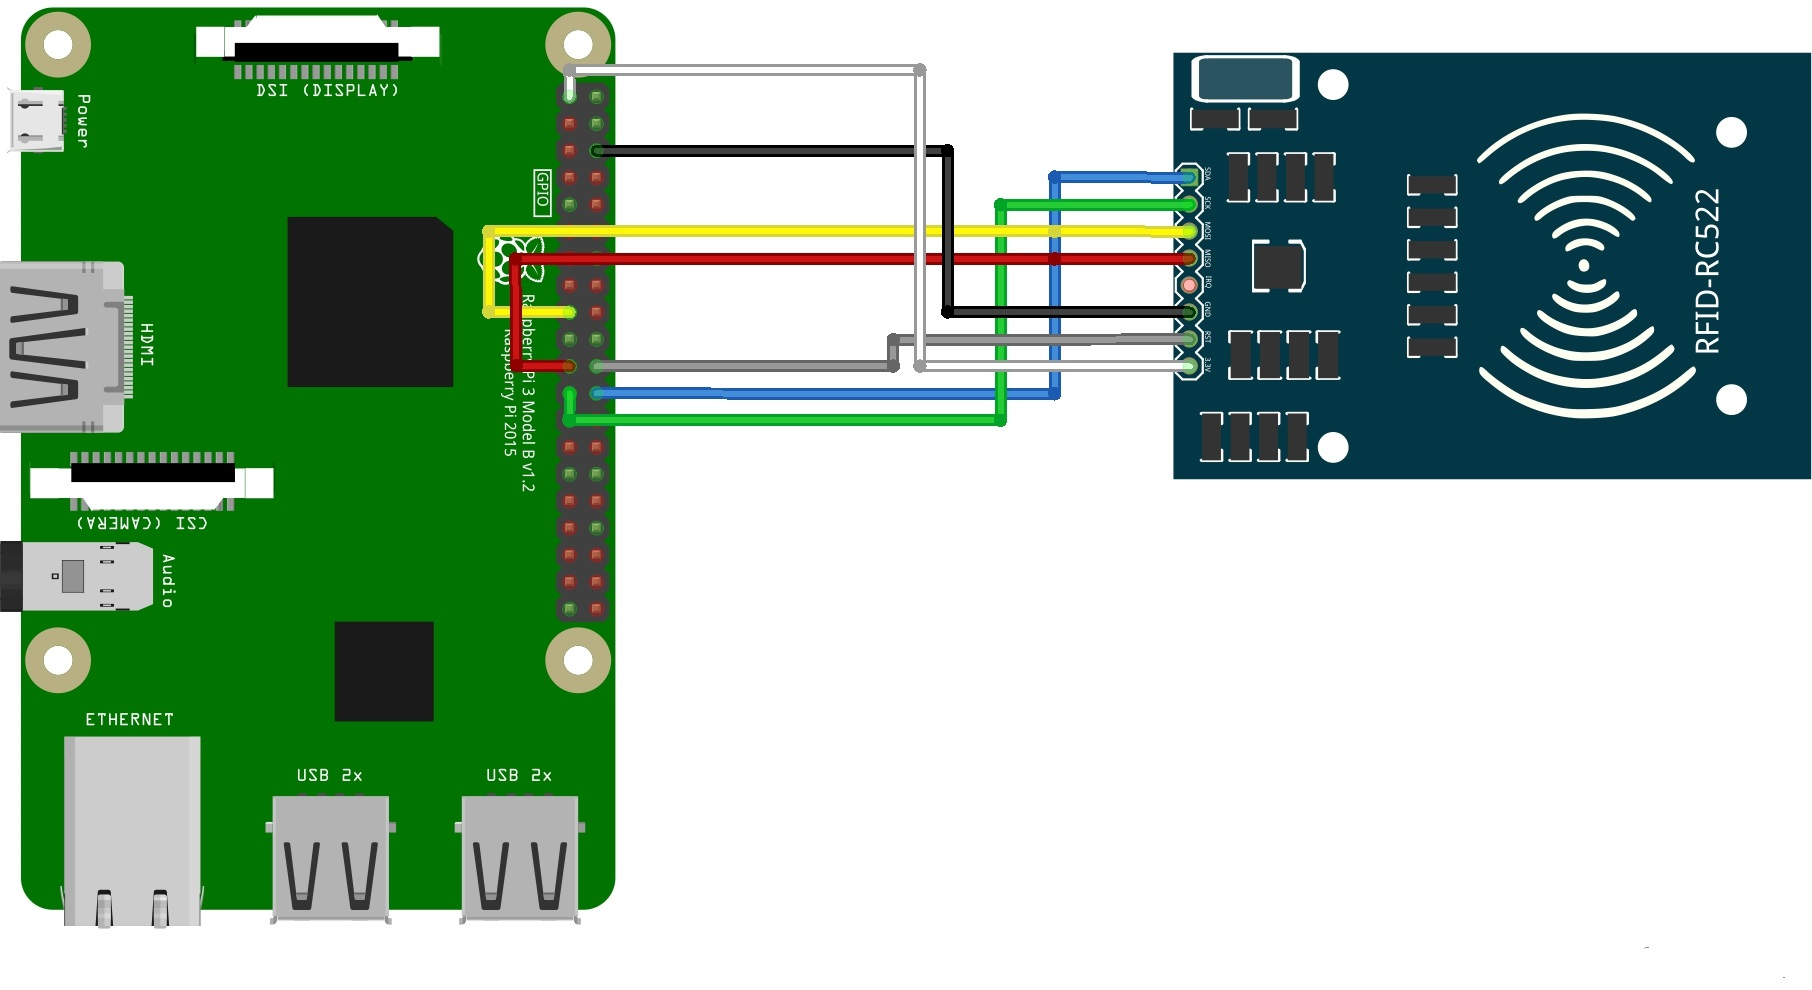
\includegraphics[width=0.85\textwidth, center]{images/skematik_rfid.jpg}
    \caption{Ragkaian Raspberry Pi dan RFID}
    \label{fig:skematikRfid}
\end{figure}

\begin{atable}
    \caption{Rangkaian pin RFID ke Raspberry Pi}
    \label{table:tableRfid}
    \csvreader[
        % column count = 11,
        tabular=cc,
        head to column names,
        before table=\rowcolors{2}{gray!15}{gray!30},
        table head= \rowcolor{gray!50!black} 
            \color{white} RFID & 
            \color{white} RASPBERRY PI 
            \\]
        {tables/tablerfid.csv}
        {
            RFID=\RFID, 
            RASPBERRYPI=\RASPBERRYPI}
        {
            \RFID & 
            \RASPBERRYPI}
\end{atable}

\subsection{Raspberry Pi dan HC-SR04}
\begin{figure} [H]
    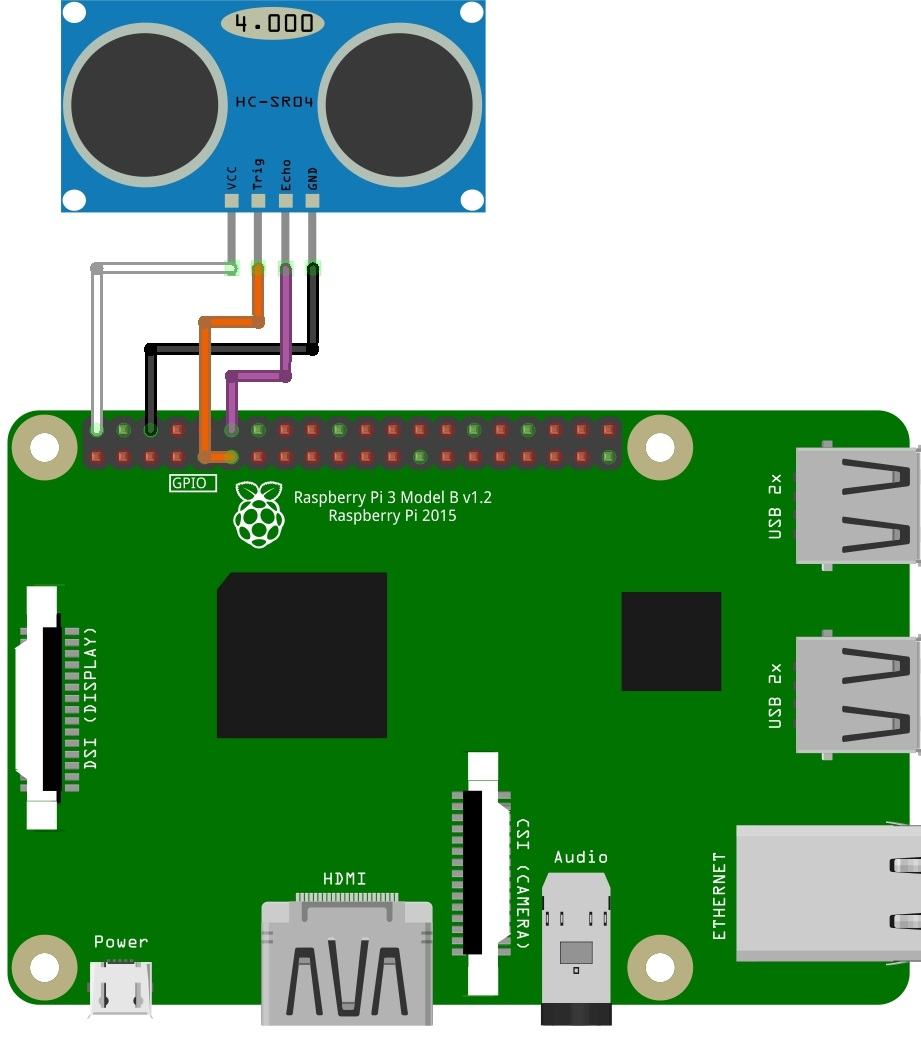
\includegraphics[height=7cm, width=0.5\textwidth, center]{images/skematik_ultra.jpg}
    \caption{Ragkaian Raspberry Pi dan Ultrasonik}
    \label{fig:skematikUltrasonik}
\end{figure}

\begin{atable}
    \caption{Rangkaian pin Ultrasonik ke Raspberry Pi}
    \label{table:tableUltrasonic}
    \csvreader[
        % column count = 11,
        tabular=cc,
        head to column names,
        before table=\rowcolors{2}{gray!15}{gray!30},
        table head= \rowcolor{gray!50!black} 
            \color{white} ULTRASONIK & 
            \color{white} RASPBERRY PI 
            \\]
        {tables/tableultrasonic.csv}
        {
            ULTRASONIC=\ULTRASONIC, 
            RASPBERRYPI=\RASPBERRYPI}
        {
            \ULTRASONIC & 
            \RASPBERRYPI}
\end{atable}

\subsection{Raspberry Pi dan SG90}
\begin{figure} [H]
    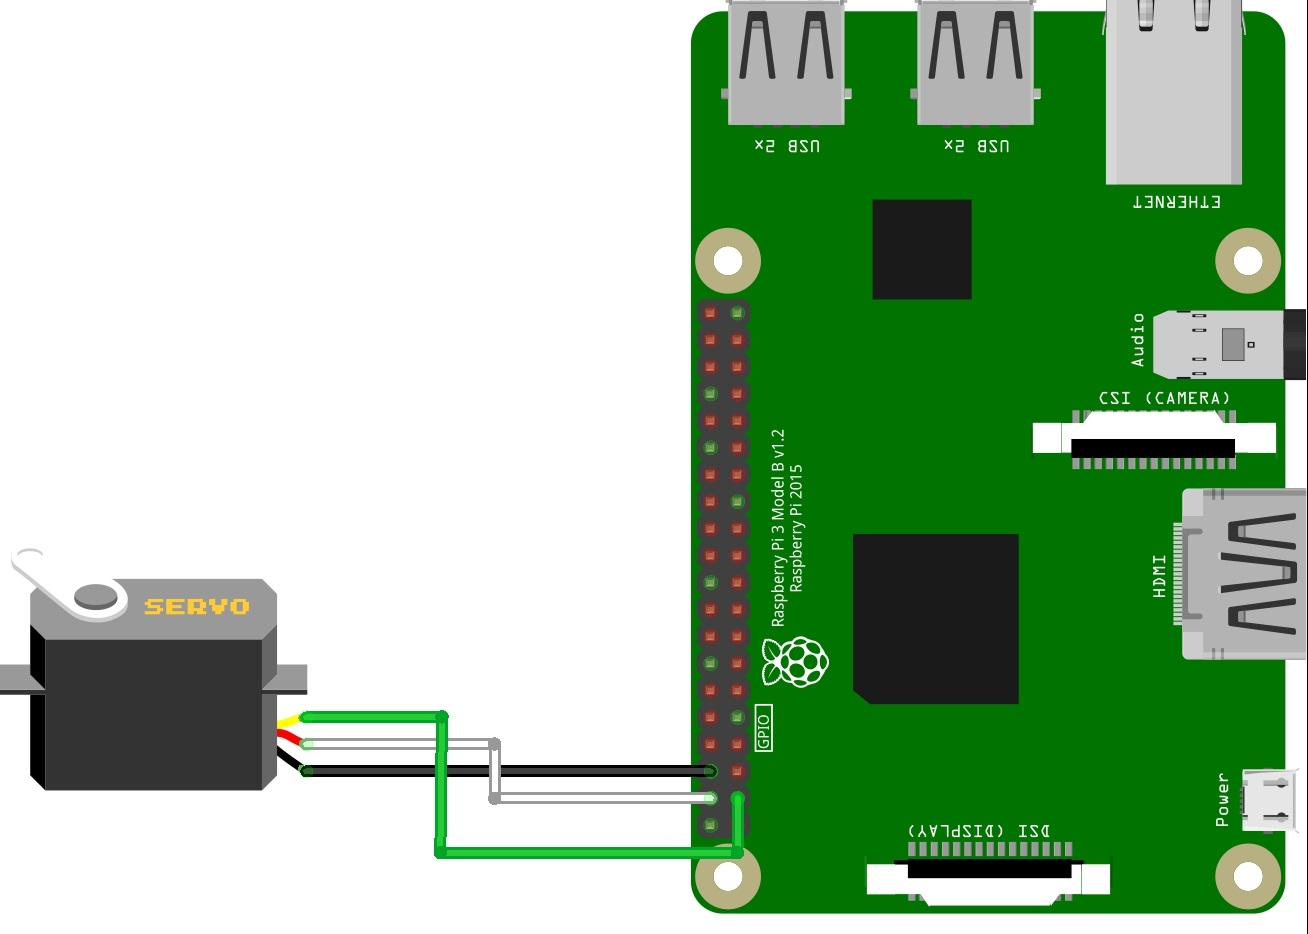
\includegraphics[height=7cm, width=0.6\textwidth, center]{images/skematik_servo.jpg}
    \caption{Ragkaian Raspberry Pi dan Servo}
    \label{fig:skematikServo}
\end{figure}

\begin{atable}
    \caption{Rangkaian pin Servo ke Raspberry Pi}
    \label{table:tableServo}
    \csvreader[
        % column count = 11,
        tabular=cc,
        head to column names,
        before table=\rowcolors{2}{gray!15}{gray!30},
        table head= \rowcolor{gray!50!black} 
            \color{white} SERVO & 
            \color{white} RASPBERRY PI 
            \\]
        {tables/tableservo.csv}
        {
            SERVO=\SERVO, 
            RASPBERRYPI=\RASPBERRYPI}
        {
            \SERVO & 
            \RASPBERRYPI}
\end{atable}

\subsection{Raspberry Pi dan Kamera Pi}

% \subsection{Hasil Perancangan Perangkat Lunak}

\section{Hasil Rancangan Aplikasi Web}

\subsection{Activity Diagram}

\subsection{Struktur \textit{Database}}
Nama \textit{database} : skripsi

Pada \textit{database} aplikasi ini, tabel dibagi menjadi 5 tabel sebagai berikut:

\begin{enumerate}[topsep=0pt,itemsep=0pt,partopsep=0pt, parsep=0pt]
    \item Tabel rfid\_tag

    Nama Tabel : rfid\_tag

    \textit{Primary Key} : id

    \begin{atable}
        \caption{rfid\_tag}
        \label{table:db_rfid_tag}
        \csvreader[
            % column count = 11,
            tabular=cc,
            head to column names,
            before table=\rowcolors{2}{gray!15}{gray!30},
            table head= \rowcolor{gray!50!black} 
                \color{white} \textit{Coloumn} & 
                \color{white} \textit{Type} 
                \\]
            {tables/db_rfid_tag.csv}
            {
                Coloumn=\Coloumn, 
                Type=\Type}
            {
                \Coloumn & 
                \Type}
    \end{atable}

    Atribut \textit{id} pada tabel rfid\_tag berfungsi sebagai kunci utama. Atribut jenis\_kendaraan digunakan untuk menentukan jenis kendaraan yang digunakan oleh pengemudi. Atribut saldo digunakan untuk menyimpan saldo dari pengemudi.

    \item Tabel tempat\_parkir

    Nama Tabel : tempat\_parkir

    \textit{Primary Key} : id

    \begin{table} [H]
        \centering
        \caption{tempat\_parkir}
        \label{table:db_tempat_parkir}
        \csvreader[
            % column count = 11,
            tabular=cc,
            head to column names,
            before table=\rowcolors{2}{gray!15}{gray!30},
            table head= \rowcolor{gray!50!black} 
                \color{white} \textit{Coloumn} & 
                \color{white} \textit{Type} 
                \\]
            {tables/db_tempat_parkir.csv}
            {
                Coloumn=\Coloumn, 
                Type=\Type}
            {
                \Coloumn & 
                \Type}
    \end{table}

    Tabel tempat\_parkir mempunyai atribut \textit{id} yang berfungsi sebagai kunci utama, atribut \textit{id} juga berfungsi sebagai nomor slot tempat parkir. Atribut jenis digunakan untuk menentukan jenis dari slot parkir. Atribut tarif digunakan sebagai tarif per jam dari slot parkir. Atribut status digunakan untuk mengetahui apakah slot sedang tersedia atau terpakai.

    \item Tabel kendaraan

    Nama Tabel : kendaraan

    \textit{Primary Key} : id

    \textit{Foreign Key} : id\_rfid\_tag

    % \begin{table} [H]
    %     \centering 
    %     \caption{kendaraan}
    %     \label{table:db_kendaraan}
    %     \csvreader[
    %         % column count = 11,
    %         tabular=cc,
    %         head to column names,
    %         before table=\rowcolors{2}{gray!15}{gray!30},
    %         table head= \rowcolor{gray!50!black} 
    %             \color{white} \textit{Coloumn} & 
    %             \color{white} \textit{Type} 
    %             \\]
    %         {tables/db_kendaraan.csv}
    %         {
    %             Coloumn=\Coloumn, 
    %             Type=\Type}
    %         {
    %             \Coloumn & 
    %             \Type}
    % \end{table}

    Tabel kendaraan mempunyai atribut \textit{id} yang berfungsi sebagai kunci utama. Atribut nomor\_plat berfungsi untuk menyimpan nomor plat pengendara. Atribut id\_rfid\_tag didapat dari tabel rfid\_tag.

    \item Tabel parkir

    Nama Tabel : parkir

    \textit{Primary Key} : id

    \textit{Foreign Key} : id\_rfid\_tag, id\_tempat\_parkir

    % \begin{table} [H]
    %     \centering
    %     \caption{parkir}
    %     \label{table:db_parkir}
    %     \csvreader[
    %         % column count = 11,
    %         tabular=cc,
    %         head to column names,
    %         before table=\rowcolors{2}{gray!15}{gray!30},
    %         table head= \rowcolor{gray!50!black} 
    %             \color{white} \textit{Coloumn} & 
    %             \color{white} \textit{Type} 
    %             \\]
    %         {tables/db_parkir.csv}
    %         {
    %             Coloumn=\Coloumn, 
    %             Type=\Type}
    %         {
    %             \Coloumn & 
    %             \Type}
    % \end{table}

    Tabel kendaraan mempunyai atribut \textit{id} yang berfungsi sebagai kunci utama. Atribut id\_rfid\_tag didapat dari tabel rfid\_tag. Atribut nomor\_plat digunakan untuk menyimpan nomor plat pengendara. Atribut id\_tempat\_parkir didapat dari tabel tempat\_parkir. Atribut waktu\_masuk digunakan untuk mencatat waktu masuk pengendara. Atribut waktu\_keluar digunakan untuk mencatat waktu keluar pengguna.

    \item Tabel \textit{reload\_id}

    Nama Tabel : reload\_id

    \textit{Primary Key} : id

    \begin{table} [H]
        \centering
        \caption{reload\_id}
        \label{table:db_reload_id}
        \csvreader[
            % column count = 11,
            tabular=cc,
            head to column names,
            before table=\rowcolors{2}{gray!15}{gray!30},
            table head= \rowcolor{gray!50!black} 
                \color{white} \textit{Coloumn} & 
                \color{white} \textit{Type} 
                \\]
            {tables/db_reload_id.csv}
            {
                Coloumn=\Coloumn, 
                Type=\Type}
            {
                \Coloumn & 
                \Type}
    \end{table}

    Tabel reload\_id mempunyai atribut \textit{id} yang berfungsi sebagai kunci utama. Atribut uid digunakan untuk menyimpan id rfid tag.

\end{enumerate}

\subsection{Tampilan Website}